\chapter{Угловой момент}

\section{Повороты и оператор углового момента. Изотропность пространства и сохранение углового момента в квантовой механике.}

\begin{figure}[h]
  \centering
  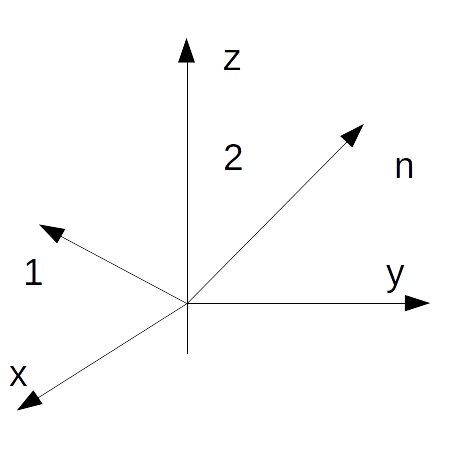
\includegraphics[scale=0.6]{figs/8_1}
  \caption{Повороты в декартовой системе координат}
  \label{fig:8_1}
\end{figure}

(поворот можно осуществлять путём подбора единичного вектора $\vec{n}$ и угла поворота $\rchi$)

$$
\ket{\psi;2} = \op{R}(\vec{\rchi}) \ket{\psi;1}
$$

$\op{R}(\vec{\rchi})$ -- оператор поворота.

Примем, что $\bk{\psi;2}{\psi;2} = \bk{\psi;1}{\psi;1}$, тогда $\op{R}^\dag \op{R} = \mathds{1}$, т.е. $\op{R}$ -- унитарный оператор.

Введём $\op{R}$ по аналогии с оператором эволюции (см. \eqref{eq:6_4_4}):
\begin{equation}
\label{eq:8_1_1}
\boxed {
	\op{R}(\op{\rchi}) \equiv e^{-(i/\hbar) \op{\vec{J}} \vec{\rchi}}
}
\end{equation}
где $\op{\vec{J}}$ -- некоторый векторный эрмитовый оператор, не зависящий от времени.

Из изотропности пространства следует, что оба состояния удовлятворяют уравнению Шрёдингера:
$$
i\hbar \pd{\ket{\psi;2}}{t} = i\hbar \op{R}(\vec{\rchi}) \pd{\ket{\psi;1}}{t} = \op{R}(\vec{\rchi}) \op{H}\ket{\psi;1}
$$

$$
i\hbar \pd{\ket{\psi;2}}{t} = \op{H}\ket{\psi;2} = \op{H} \op{R}(\vec{\rchi}) \ket{\psi;1}
$$

Сравнивая правые части, легко видеть, что $\brs{\op{H}, \op{R}(\vec{\rchi})} = 0$

Распишем экспоненту в \eqref{eq:8_1_1} в виде ряда:
$$
\op{R}(\vec{\rchi}) = \sum_{k=0}^{\infty} \frac{1}{k!} \brc{- \frac{i}{\hbar} \op{\vec{J}} \vec{\rchi}}^k
$$

Подставляя её в условие коммутации, получим:
\begin{equation}
\label{eq:8_1_2}
\boxed {
	\brs{\op{H}, \op{\vec{J}}} = 0
}
\end{equation}

\begin{excr}
доказать \eqref{eq:8_1_2}
\end{excr}

$\vec{J}$ -- интеграл движения (см. \S 9 т.1 Л-Л <<Сохранение углового момента>>)

$\op{\vec{J}}$ -- \textbf{оператор углового момента} ($\op{\vec{J}} = \brcr{\op{L}, \op{S}, \op{L}+\op{S}}$, где $\op{L}$ -- оператор орбитального момента, $\op{S}$ --оператор спинового момента, $(\op{L} + \op{S})$ -- полный момент)

\begin{sloppypar}
  \section{Коммутационные соотношения для оператора углового момента. Система собственных векторов операторов \texorpdfstring{$\op{\vec{j}}^2$ и $\op{\vec{j}_z}$}{углового момента}}
\end{sloppypar}

Обозначим: $\boxed{\op{\vec{j}} = \frac{\op{\vec{J}}}{\hbar}}$

\begin{defn}
Векторный оператор $\op{\vec{j}} = \brcr{\op{j_x}, \op{j_y}, \op{j_z}}$ называют \textbf{оператором углового момента}, если все его компоненты являются \textbf{наблюдаемыми} (эрмитовыми) и удовлетворяют коммутационным соотношениям:
\begin{equation}
\label{eq:8_2_1}
\boxed {
	\brs{\op{j_i}, \op{j_k}} = i e_{ikl} \op{j_l}
}
\end{equation}
(где $e_{ikl}$ -- антисимметричный тензор)
\end{defn}

$$
\op{\vec{j}}^2 = \op{j_x}^2 + \op{j_y}^2 + \op{j_z}^2
$$

Совместная измеримость $\op{j}^2$ возможна только с одной компонентой:
\begin{equation}
\label{eq:8_2_2}
\brs{\op{j}^2, \op{j_i}} = 0
\end{equation}

\begin{excr}
Доказать \eqref{eq:8_2_2} с помощью \eqref{eq:8_2_1}
\end{excr}

$\ket{jm}$ - полная общая система собственных векторов:
\begin{equation}
\label{eq:8_2_3}
\left\{
\begin{aligned}
\op{\vec{j}}^2 \ket{jm} = \lambda(j) \ket{jm} \\
\op{\vec{j}}_z \ket{jm} = m \ket{jm}
\end{aligned}
\right.
\end{equation}

Условие ортонормировки:
$$
\bk{jm}{j'm'} = \delta_{jj'} \delta{mm'}
$$

$$
\avg{\op{\vec{j}}^2} = \avg{\op{j_x}^2} + \avg{\op{j_y}^2} + \avg{\op{j_z}^2} \geqslant \avg{\op{j_z}^2}
$$

То есть:
$$
\lambda(j) \geqslant m^2 ~~\rightarrow~~ \left\{
\begin{aligned}
m_{min} &\leqslant m \leqslant m_{max}\\
m_{max} &= - m_{min}
\end{aligned}
\right.
$$

$m_{max} \equiv j$, тогда $m_{min} = -j$

Обозначим:
\begin{equation}
\label{eq:8_2_4}
\left\{
\begin{aligned}
\op{j}_{+} &= \op{j}_{x} + i \op{j}_{y} \\
\op{j}_{-} &= \op{j}_{x} - i \op{j}_{y} = \brc{\op{j}_{+}}^\dag
\end{aligned}
\right.
\end{equation}

\begin{equation}
\label{eq:8_2_5}
\brs{\op{j_z}, \op{j}_{\pm}} = \pm \op{j_{\pm}}
\end{equation}

\begin{excr}
Доказать \eqref{eq:8_2_5} с использованием \eqref{eq:8_2_4} и \eqref{eq:8_2_1}
\end{excr}

Из \eqref{eq:8_2_5}:
$$
\op{j_z} \brc{\op{j}_{\pm} \ket{jm}} = \brc{\op{j}_{\pm} \op{j_z} \pm \op{j}_{\pm}} \ket{jm} = (m \pm 1) \brc{\op{j}_{\pm} \ket{jm}}
$$

Будем называть $\op{j}_{+}$ \textbf{оператором повышения}, а $\op{j}_{-}$ -- \textbf{оператором понижения}

\begin{equation}
\label{eq:8_2_6}
\left\{
\begin{aligned}
\op{j}_{+} \ket{j, m-1} &= \alpha_m \ket{j, m}\\
\op{j}_{-} \ket{j, m} &= \beta_m \ket{j, m-1}\\
\end{aligned}
\right.
\end{equation}

Заметим, что:
$$
\begin{gathered}
\op{j}_{+} \ket{jj} = 0,~~\text{или}~~ \alpha_{j+1} = 0\\
\op{j}_{-} \ket{j, -j} = 0,~~\text{или}~~ \beta_{-j} = 0
\end{gathered}
$$

Цепочка понижения:
$$
\left\downarrow
\begin{aligned}
\op{j}_{-} \ket{jj} & \sim \ket{j, j-1}\\
(\op{j}_{-})^2 \ket{jj} & \sim \ket{j, j-2}\\
\cdots \\
(\op{j}_{-})^N \ket{jj} & \sim \ket{j, j-N},~~~N \in \mathbb{N} \cup \brcr{0} \\
\end{aligned}
\right.
$$

$j - N = -j$, т.е. $j = \frac{N}{2}$, следовательно $j$ принимает только целые и полуцелые значения:
$$
j = 0, \frac{1}{2}, 1, \frac{3}{2} \cdots
$$

Если $j$ фиксировано:
$$
\underbrace{m = -j, -j + 1, \cdots, j}_{(2j + 1)~\text{значения}}
$$

\noindent
$j$ -- квантовое число момента количества движения частицы\\
$m$ -- магнитное квантовое число

Значение $\lambda(j)$ пока неизвестно. При его определении будем считать, что \\
$m_{max} = -m_{min} = j$.

$$
\op{j}_{-} \op{j}_{+} \ket{jj} = 0
$$
$$
\op{j}_{-} \op{j}_{+} = \op{\vec{j}}^2 - \op{j_z}^2 - \op{j_z}
$$
\begin{excr}
Доказать предыдущее равенство используя \eqref{eq:8_2_4} и \eqref{eq:8_2_1}
\end{excr}

$$
\brc{\op{\vec{j}}^2 - \op{j_z}^2 - \op{j_z}} \ket{jj} = 0 ~~\rightarrow~~ \lambda(j) = j(j+1)
$$

\begin{equation}
\label{eq:8_2_7}
\boxed {
	\op{\vec{j}}^2 \ket{jm} = j(j+1) \ket{jm}
}
\end{equation}

Из \eqref{eq:8_2_6}:
$$
\alpha_m = \bfk{jm}{\op{j}_{+}}{j, m-1} = \bk{\op{j}_{-}jm}{j, m-1} = \left. \bfk{j,m-1}{\op{j}_{-}}{jm}^* \right|_{\text{\eqref{eq:8_2_6}}} = \beta_m^*
$$

Теперь необходимо найти $\beta_{-j+1}, \beta_{-j+2}, \cdots, \beta_{j}$

$$
\left. \op{j}_{+} \op{j}_{-} \ket{jm} \right|_{\text{\eqref{eq:8_2_6}}} = \beta_m \op{j}_{+} \ket{j, m-1} = \abs{\beta_m}^2 \ket{jm}
$$

С другой стороны:
$$
\op{j}_{+} \op{j}_{-} = \op{j}^2 - \op{j_z}^2 + \op{j_z}
$$

\begin{excr}
Доказать предыдущее равенство используя \eqref{eq:8_2_4} и \eqref{eq:8_2_1}
\end{excr}

$$
\op{j}_{+} \op{j}_{-} \ket{jm} = \left. (\op{j}^2 - \op{j_z}^2 + \op{j_z}) \ket{jm} \right|_{\text{\eqref{eq:8_2_7}, \eqref{eq:8_2_3}}} = \brc{j(j+1) - m^2 + m} \ket{jm}
$$

Фазу $\ket{jm}$ можно подобрать так, чтобы $\alpha_m = \beta_m  = \abs{\beta_m}$

$$
\beta_m = \sqrt{j^2 + j - m^2 + m} = \sqrt{(j+m)(j-m+1)} = \alpha_m
$$

$$
\begin{gathered}
\op{j}_{-} \ket{jm} = \sqrt{(j+m)(j-m+1)} \ket{j, m-1} \\
\op{j}_{+} \ket{jm} = \beta_{m+1} \ket{j, m+1} = \sqrt{(j-m)(j+m+1)} \ket{j, m+1}
\end{gathered}
$$

\begin{equation}
\label{eq:8_2_8}
\boxed {
	(\op{j_x} \pm i \op{j_y}) \ket{jm} = \sqrt{(j \mp m)(j \pm m + 1)} \ket{j, m \pm 1}
}
\end{equation}


\section{Спин частицы. Матрицы Паули.}

Спиновый оператор:
$$
\op{\vec{s}} = \brcr{\op{s}_x, \op{s}_y, \op{s}_z}
$$

будем рассматривать частицу с $s = 1/2$:

\begin{equation}
\label{eq:8_3_1}
\left\{
\begin{array}{l}
\op{\vec{s}}^2 \ket{s, m_s} = s(s+1) \ket{s, m_s}\\
\op{\vec{s}}_z \ket{s, m_s} = m_s \ket{s, m_s}
\end{array}
\right.
\end{equation}

$2s + 1 = 2$:~~ $m_s = \pm 1/2$

\begin{equation}
\label{eq:8_3_2}
  \begin{array}{l}
  \chi_{\frac{1}{2}, m_s} \equiv \ket{\frac{1}{2}, m_s}\\
  \chi_{\frac{1}{2}, \frac{1}{2}} \equiv \ket{\frac{1}{2}, \frac{1}{2}} \equiv \begin{pmatrix} 1 \\ 0 \end{pmatrix}    \equiv \ket{\alpha} \equiv \ket{+}\\
  \chi_{\frac{1}{2}, -\frac{1}{2}} \equiv \ket{\frac{1}{2}, -\frac{1}{2}} \equiv \begin{pmatrix} 0 \\ 1 \end{pmatrix}   \equiv \ket{\beta} \equiv \ket{-}
\end{array}
\end{equation}

$\ket{\alpha}$ и $\ket{\beta}$ -- базисные векторы спиновых состояний.

\begin{equation}
\label{eq:8_3_3}
\boxed{
	\ket{\chi} = a_{+} \begin{pmatrix} 1 \\ 0 \end{pmatrix} + a_{-} \begin{pmatrix} 0 \\ 1 \end{pmatrix} = \begin{pmatrix} a_{+} \\ a_{-} \end{pmatrix}
}
\end{equation}
где $a_{-}$ и $a_{+}$ -- вероятности обнаружить проекцию в $s_z = -1/2$ и $1/2$ соответственно.

$$
\avg{\chi, \chi} = 1 ~~\rightarrow ~~ \abs{a_{+}}^2 + \abs{a_{-}}^2 = 1
$$

\section{Оператор орбитального момента частицы в координатном представлении (декартовы и сферические координаты).}

$$
\vec{L} = \vr \times \vp
$$

По принципу соответствия между классической механикой и квантовой:

\begin{equation}
\label{eq:8_4_1}
  \vec{L} \to \boxed{\op{\vec{L}} = \hbar \op{\vec{l}} = \op{\vr} \times \op{\vp}}
\end{equation}

\begin{equation}
\label{eq:8_4_2}
  \op{\vec{L}} = \hbar \op{\vec{l}} = -i\hbar(\vr \times \nabla)
\end{equation}

$$
\op{\vec{l}} = \frac{\op{\vec L}}{\hbar} = -i(\vr \times \nabla) = -i \left| 
  \begin{matrix}
  \vec{i} & \vec{j} & \vec{k}\\
  x & y & z\\
  \pd{}{x} & \pd{}{y} & \pd{}{z}\\
  \end{matrix}
  \right |
$$
- \underline{безразмерный оператор орбитального момента}.
$$
\op{\vec l} = \brcr{\vec{l}_x, \vec{l}_y, \vec{l}_z} \to \vec{l}_z = -i \brc{x \pd{}{y} - y \pd{}{x}}
$$

Иначе можно записать:
\begin{equation}
\label{eq:8_4_3}
  \vec{l}_\alpha = -i e_{\alpha \beta \gamma} x_\beta \pd{}{x_\gamma},~\alpha, \beta, \gamma = 1, 2, 3
\end{equation}

Из \eqref{eq:8_4_3} получим:
\begin{equation}
\label{eq:8_4_4}
  [\op{l}_\alpha, \op{l}_\beta] = i e_{\alpha \beta \gamma} \op{l}_\gamma
\end{equation}

$$
\op{\vec{l}}^2 = \op{l}^2_x + \op{l}^2_y + \op{l}^2_z
$$

Подставим в \eqref{eq:8_4_4}: 
\begin{equation}
\label{eq:8_4_5}
  \boxed{[\op{\vec{l}}^2, \op{l}_\alpha] = 0}.
\end{equation}

Это аналог \eqref{eq:8_2_2} в теории углового момента.

\begin{figure}[h]
  \centering
  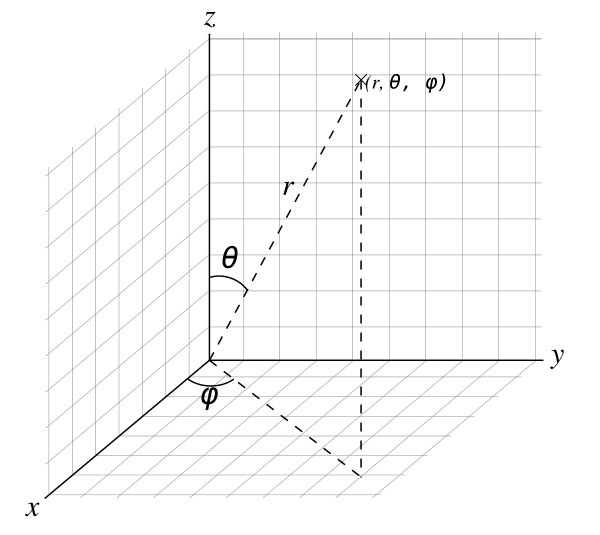
\includegraphics[scale=0.6]{figs/8_2}
  \caption{Сферическая система координат}
  \label{fig:8_2}
\end{figure}


$$
x = r \sin \theta \cos \phi
$$
$$
y = r \sin \theta \sin \phi
$$
$$
z = r \cos \theta
$$
$$
0 \le r \le \infty,~~~0 \le \theta \le \pi, ~~~ 0 \le \phi \le 2\pi
$$
Запишем частную производную по углу $\phi$:
$$
\pd{}{\phi} =\underbrace{\pd{x}{\phi}}_{-r \sin \theta \sin \phi}\cdot \pd{}{x} + \underbrace{\pd{y}{\phi}}_{r \sin \theta \cos \phi}\cdot \pd{}{y} + \underbrace{\pd{z}{\phi}}_{=0} \cdot \pd{}{z}
$$ 

Получим:
$$
\pd{}{\phi} = x \pd{}{y} - y \pd{}{x}
$$
$$
\boxed{\op{l}_z = -i \pd{}{\phi}}
$$

Аналогично можно получить выражения для других компонент орбитального момента:
$$
\op{l}_x = -i(-\sin \phi \pd{}{\theta} - \cos \phi \ctg \theta \pd{}{\phi})
$$
$$
\op{l}_y = -i(\cos \phi \pd{}{\theta} - \sin \phi \ctg \theta \pd{}{\phi})
$$
$$
\op{\vec{l}}^2 = -\brs{ \frac{1}{\sin \theta} \pd{}{\theta} \brc{\sin \theta \pd{}{\theta}} + \frac{1}{\sin \theta} \pd{^2}{\phi^2}} = - \Delta_{\theta, \phi}
$$
Введем лапласиан в сферических координатах:
$$
\Delta_{\vr} = \underbrace{\frac{1}{r^2} \pd{}{r} \brc{r^2 \pd{}{r}}}_{\text{радиальная часть}} + \underbrace{ \frac{1}{r^2} \Delta_{\theta, \phi}}_{\text{угловая часть}}
$$
\begin{equation}
\label{eq:8_4_6}
\op{H} = - \frac{\hbar^2}{2m} \brc{\frac{1}{r^2} \pd{}{r} \brc{r^2 \pd{}{r}} - \frac{\vec{l}^2}{r^2}} + U(\vr)
\end{equation}

\section{Сферические гармоники}

Запишем уравнение на собственные функции оператора $\op{l}_z$:

\begin{equation}
\label{eq:8_5_1}
-i \pd{}{\phi} \underbrace{\bk{\phi}{m}}_{=\Phi_m(\phi)} = m \bk{\phi}{m}
\end{equation}

Здесь 
\begin{equation}
\label{eq:8_5_2}
  \Phi_m(\phi) = C e^{i m \phi}
\end{equation}

Найдем возможные значения $m$:
$$
\phi \to \phi + 2\pi ~:~\Phi_m(\phi) = \Phi_m(\phi + 2\pi) \Rightarrow 
$$
$$
e^{im2\pi} = 1 \Rightarrow \boxed{m=0, \pm 1, \pm 2, ...}
$$

Константа $C$ определяется из условия нормировки:

$$
C = \frac{1}{\sqrt{2\pi}} \Rightarrow \int_0^{2\pi} d\phi \Phi^*_m(\phi) \Phi_{m'}(\phi) = \delta_{mm'} 
$$
Запишем задачу на собственные значения $\op{l}_z$ и $\op{\vec l}^2$:
\begin{equation}
\label{eq:8_5_3}
\left\{
  \begin{matrix}
    \op{\vec{l}}^2 \ket{lm} = l(l+1)\ket{lm} \\
    \op{l}_z \ket{lm} = m \ket{lm}
  \end{matrix}
\right.
\end{equation}


\begin{equation}
\left\{
  \begin{matrix}
  \label{eq:8_5_3_add}
   - \Delta_{\theta, \phi} Y_{lm}(\theta, \phi) = l(l+1) Y_{lm}(\theta, \phi) 
    \\
     -i\pd{}{\phi} Y_{lm}(\theta, \phi) = m Y_{lm}(\theta, \phi) 
  \end{matrix}
\right .
\end{equation}
  
$Y_{lm}(\theta, \phi)$ - сферические функции(сферические гармоники), решения задачи на собственные функции для $\op{l}_z$ и $\op{\vec l}^2$ в сферических координатах.

Проекция $\ket{lm}$ на $(\theta, \phi)$ : $Y_{lm}(\theta, \phi) = \bk{\theta \phi}{lm}$.

Найдем явный вид сферических функций. Для этого воспользуемся методом разделения переменных:
$$
Y_{lm}(\theta, \phi) = \theta_{lm}(\theta) \Phi_m(\phi)
$$
Подставляя в \eqref{eq:8_5_3_add} можно получить уравнение на $\theta_{lm}(\theta)$. В итоге получим:
$$
\boxed{Y_{lm}(\theta, \phi) = C_{lm} e^{im\phi} P^m_l(\cos \theta)}
$$

$ P^m_l(\cos \theta)$ - присоединенные полиномы Лежандра.

$$
l = \abs{m}, \abs{m} + 1, ..., ~~~(l \ge \abs{m})
$$
 
Для $l = 0, 1, 2, ...$ $m = 0, \pm 1, \pm 2, ..., \pm l$.

$$
\begin{matrix}
l =  & 0 & 1 & 2 & 3 & ... & \\
       & s & p & d & f & ... & \text{- состояния}
\end{matrix}
$$
$$
\boxed{\bk{Y_{lm}}{Y_{l'm'}} = \int_0^{2\pi} d\phi \int_0^\pi \sin \theta d \theta Y^*_{lm}(\theta, \phi) Y_{l'm'}(\theta, \phi) = \delta_{ll'} \delta_{mm'}}
$$
\begin{equation}
\label{8_5_4}
(r = 1, \theta \in [0, \pi], \phi \in [0, 2\pi]) -
\end{equation}
полный ортонормированный базис.